\documentclass[border=10pt,tikz]{standalone}
\usepackage[utf8]{inputenc}
\usepackage{tikz}
\usetikzlibrary{arrows.meta, positioning}
\usepackage{xcolor}

\definecolor{cGreen}{HTML}{27AE60}
\definecolor{cRed}{HTML}{C0392B}
\definecolor{cGray}{HTML}{7F8C8D}
\definecolor{cPurple}{HTML}{8E44AD}

\begin{document}
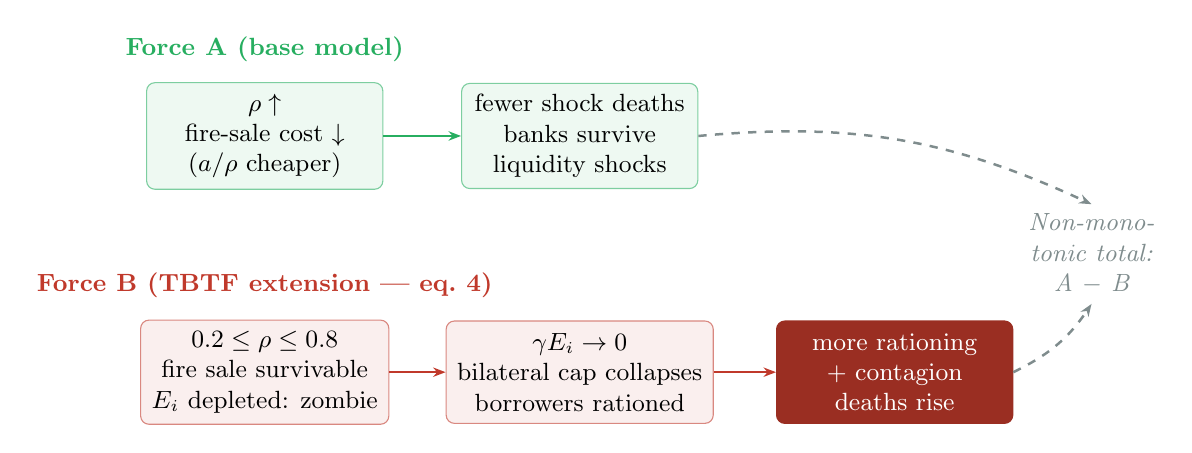
\begin{tikzpicture}[
  force/.style={rectangle, rounded corners=3pt, draw, minimum width=3cm,
                minimum height=1.3cm, align=center, font=\small, inner sep=4pt},
  greenbox/.style={force, fill=cGreen!8, draw=cGreen!60},
  redbox/.style={force, fill=cRed!8, draw=cRed!60},
  darkred/.style={force, fill=cRed!80!black, draw=cRed!80!black, text=white},
  arr/.style={-{Stealth[length=4.5pt]}, line width=0.9pt},
]

% ---- Row A (top) ----
\node[font=\small\bfseries, color=cGreen] (la) at (0,0) {Force A (base model)};
\node[greenbox] (ga1) at (0,-1.1) {$\rho\uparrow$\\fire-sale cost $\downarrow$\\$(a/\rho$ cheaper)};
\node[greenbox] (ga2) at (4,-1.1) {fewer shock deaths\\banks survive\\liquidity shocks};
\draw[arr, color=cGreen] (ga1) -- (ga2);

% ---- Row B (bottom) ----
\node[font=\small\bfseries, color=cRed] (lb) at (0,-3.0)
  {Force B (TBTF extension --- eq.~4)};
\node[redbox] (gb1) at (0,-4.1)  {$0.2 \leq \rho \leq 0.8$\\fire sale survivable\\$E_i$ depleted: zombie};
\node[redbox] (gb2) at (4,-4.1)  {$\gamma E_i \to 0$\\bilateral cap collapses\\borrowers rationed};
\node[darkred] (gb3) at (8,-4.1) {more rationing\\+ contagion\\deaths rise};
\draw[arr, color=cRed] (gb1) -- (gb2);
\draw[arr, color=cRed] (gb2) -- (gb3);

% ---- Summary node ----
\node[font=\small\itshape, color=cGray, align=center] (sum) at (10.5,-2.6)
  {Non-mono-\\tonic total:\\A $-$ B};
\draw[arr, color=cGray, dashed] (ga2.east) to[bend left=15]  (sum.north);
\draw[arr, color=cGray, dashed] (gb3.east) to[bend right=15] (sum.south);

\end{tikzpicture}
\end{document}
